% Please have a look at the README.md file for info on how to use the template
%\documentclass[a4paper,12pt,times,numbered,print,index]{Classes/PhDThesisPSnPDF}

%documentclass[a4grep -n 'addbibresource' Preamble/preamble.tex
%paper,12pt,times,custombib,print,index]{Classes/PhDThesisPSnPDF}

%\documentclass[a4paper,12pt,times,custombib,print,index]{Classes/PhDThesisPSnPDF}

\documentclass[a4paper,12pt,times,custombib,print,index]{Classes/PhDThesisPSnPDF}

% ******************************************************************************
% ******************************* Class Options ********************************
% *********************** See README for more details **************************
% ******************************************************************************

% `a4paper'(The University of Cambridge PhD thesis guidelines recommends a page
% size a4 - default option) or `a5paper': A5 Paper size is also allowed as per
% the Cambridge University Engineering Deparment guidelines for PhD thesis
%
% `11pt' or `12pt'(default): Font Size 10pt is NOT recommended by the University
% guidelines
%
% `oneside' or `twoside'(default): Printing double side (twoside) or single
% side.
%
% `print': Use `print' for print version with appropriate margins and page
% layout. Leaving the options field blank will activate Online version.
%
% `index': For index at the end of the thesis
%
% `draftclassic': For draft mode without loading any images (same as draft in book)
%
% `draft': Special draft mode with line numbers, images, and water mark with
% timestamp and custom text. Position of the text can also be modified.
%
% `abstract': To generate only the title page and abstract page with
% dissertation title and name, to submit to the Student Registry
%
% `chapter`: This option enables only the specified chapter and it's references
%  Useful for review and corrections.
%
% ************************* Custom Page Margins ********************************
%
% `custommargin`: Use `custommargin' in options to activate custom page margins,
% which can be defined in the preamble.tex. Custom margin will override
% print/online margin setup.
%
% *********************** Choosing the Fonts in Class Options ******************
%
% `times' : Times font with math support. (The Cambridge University guidelines
% recommend using times)
%
% `fourier': Utopia Font with Fourier Math font (Font has to be installed)
%            It's a free font.
%
% `customfont': Use `customfont' option in the document class and load the
% package in the preamble.tex
%
% default or leave empty: `Latin Modern' font will be loaded.
%
% ********************** Choosing the Bibliography style ***********************
%
% `authoryear': For author-year citation eg., Krishna (2013)
%
% `numbered': (Default Option) For numbered and sorted citation e.g., [1,5,2]
%
% `custombib': Define your own bibliography style in the `preamble.tex' file.
%              `\RequirePackage[square, sort, numbers, authoryear]{natbib}'.
%              This can be also used to load biblatex instead of natbib
%              (See Preamble)
%
% **************************** Choosing the Page Style *************************
%
% `default (leave empty)': For Page Numbers in Header (Left Even, Right Odd) and
% Chapter Name in Header (Right Even) and Section Name (Left Odd). Blank Footer.
%
% `PageStyleI': Chapter Name next & Page Number on Even Side (Left Even).
% Section Name & Page Number in Header on Odd Side (Right Odd). Footer is empty.
%
% `PageStyleII': Chapter Name on Even Side (Left Even) in Header. Section Number
% and Section Name in Header on Odd Side (Right Odd). Page numbering in footer

% Uncomment to change page style
%\pagestyle{PageStyleII}

% ********************************** Preamble **********************************
% Preamble: Contains packages and user-defined commands and settings
% ******************************************************************************
% ****************************** Custom Margin *********************************

% Add `custommargin' in the document class options to use this section
% Set {innerside margin / outerside margin / topmargin / bottom margin}  and
% other page dimensions
\ifsetCustomMargin
  \RequirePackage[left=37mm,right=30mm,top=35mm,bottom=30mm]{geometry}
  \setFancyHdr % To apply fancy header after geometry package is loaded
\fi

% Add spaces between paragraphs
%\setlength{\parskip}{0.5em}
% Ragged bottom avoids extra whitespaces between paragraphs
\raggedbottom
% To remove the excess top spacing for enumeration, list and description
%\usepackage{enumitem}
%\setlist[enumerate,itemize,description]{topsep=0em}

% *****************************************************************************
% ******************* Fonts (like different typewriter fonts etc.)*************

% Add `customfont' in the document class option to use this section

\ifsetCustomFont
  % Set your custom font here and use `customfont' in options. Leave empty to
  % load computer modern font (default LaTeX font).
  %\RequirePackage{helvet}

  % For use with XeLaTeX
  %  \setmainfont[
  %    Path              = ./libertine/opentype/,
  %    Extension         = .otf,
  %    UprightFont = LinLibertine_R,
  %    BoldFont = LinLibertine_RZ, % Linux Libertine O Regular Semibold
  %    ItalicFont = LinLibertine_RI,
  %    BoldItalicFont = LinLibertine_RZI, % Linux Libertine O Regular Semibold Italic
  %  ]
  %  {libertine}
  %  % load font from system font
  %  \newfontfamily\libertinesystemfont{Linux Libertine O}
\fi

% *****************************************************************************
% **************************** Custom Packages ********************************

% ************************* Algorithms and Pseudocode **************************

\usepackage{algpseudocode}


% ********************Captions and Hyperreferencing / URL **********************




% Captions: This makes captions of figures use a boldfaced small font.
%\RequirePackage[small,bf]{caption}

\RequirePackage[labelsep=space,tableposition=top]{caption}
\renewcommand{\figurename}{Fig.} %to support older versions of captions.sty


% *************************** Graphics and figures *****************************

%\usepackage{rotating}
%\usepackage{wrapfig}

% Uncomment the following two lines to force Latex to place the figure.
% Use [H] when including graphics. Note 'H' instead of 'h'
%\usepackage{float}
%\restylefloat{figure}

% Subcaption package is also available in the sty folder you can use that by
% uncommenting the following line
% This is for people stuck with older versions of texlive
%\usepackage{sty/caption/subcaption}
\usepackage{subcaption}

% ********************************** Tables ************************************
\usepackage{booktabs} % For professional looking tables
\usepackage{multirow}

%\usepackage{multicol}
%\usepackage{longtable}
%\usepackage{tabularx}


% *********************************** SI Units *********************************
\usepackage{siunitx} % use this package module for SI units


% ******************************* Line Spacing *********************************

% Choose linespacing as appropriate. Default is one-half line spacing as per the
% University guidelines

% \doublespacing
% \onehalfspacing
% \singlespacing


% ************************ Formatting / Footnote *******************************

% Don't break enumeration (etc.) across pages in an ugly manner (default 10000)
%\clubpenalty=500
%\widowpenalty=500

%\usepackage[perpage]{footmisc} %Range of footnote options


% *****************************************************************************
% *************************** Bibliography  and References ********************

%\usepackage{cleveref} %Referencing without need to explicitly state fig /table

% Add `custombib' in the document class option to use this section
%\ifuseCustomBib
   %\RequirePackage[square, sort, numbers, authoryear]{natbib} % CustomBib

% If you would like to use biblatex for your reference management, as opposed to the default `natbibpackage` pass the option `custombib` in the document class. Comment out the previous line to make sure you don't load the natbib package. Uncomment the following lines and specify the location of references.bib file


%\usepackage[backend=biber, style=numeric-comp, citestyle=numeric, natbib=true, sorting=nty]{biblatex}
%\usepackage[backend=biber, style=numeric-comp, sorting=nty]{biblatex}

%\usepackage[backend=biber,style=numeric-comp,citestyle=numeric,natbib=true,sorting=nty]{biblatex}
\usepackage[backend=biber,style=numeric-comp,citestyle=numeric,natbib=true,sorting=nty,refsection=none]{biblatex}

\addbibresource{References/references.bib}


%\RequirePackage[backend=biber, style=numeric-comp, citestyle=numeric, sorting=nty, natbib=true]{biblatex}
%\bibliography{References/references} %Location of references.bib only for biblatex


% changes the default name `Bibliography` -> `References'
\renewcommand{\bibname}{References}


% ******************************************************************************
% ************************* User Defined Commands ******************************
% ******************************************************************************

% *********** To change the name of Table of Contents / LOF and LOT ************

%\renewcommand{\contentsname}{My Table of Contents}
%\renewcommand{\listfigurename}{My List of Figures}
%\renewcommand{\listtablename}{My List of Tables}


% ********************** TOC depth and numbering depth *************************

\setcounter{secnumdepth}{2}
\setcounter{tocdepth}{3}


% ******************************* Nomenclature *********************************

% To change the name of the Nomenclature section, uncomment the following line

%\renewcommand{\nomname}{Symbols}


% ********************************* Appendix ***********************************

% The default value of both \appendixtocname and \appendixpagename is `Appendices'. These names can all be changed via:

%\renewcommand{\appendixtocname}{List of appendices}
%\renewcommand{\appendixname}{Appndx}

% *********************** Configure Draft Mode **********************************

% Uncomment to disable figures in `draft'
%\setkeys{Gin}{draft=true}  % set draft to false to enable figures in `draft'

% These options are active only during the draft mode
% Default text is "Draft"
%\SetDraftText{DRAFT}

% Default Watermark location is top. Location (top/bottom)
%\SetDraftWMPosition{bottom}

% Draft Version - default is v1.0
%\SetDraftVersion{v1.1}

% Draft Text grayscale value (should be between 0-black and 1-white)
% Default value is 0.75
%\SetDraftGrayScale{0.8}


% ******************************** Todo Notes **********************************
%% Uncomment the following lines to have todonotes.

%\ifsetDraft
%	\usepackage[colorinlistoftodos]{todonotes}
%	\newcommand{\mynote}[1]{\todo[author=kks32,size=\small,inline,color=green!40]{#1}}
%\else
%	\newcommand{\mynote}[1]{}
%	\newcommand{\listoftodos}{}
%\fi

% Example todo: \mynote{Hey! I have a note}
\usepackage[table]{xcolor}
\usepackage{colortbl}

\usepackage{graphicx}
\usepackage{hyperref}  % add this in the preamble
\newcommand{\geno}[1]{\textnormal{#1}}
\usepackage{booktabs}
\usepackage{colortbl}
\usepackage{array}
\usepackage{adjustbox}


    \usepackage{booktabs}
    \usepackage{graphicx}   % for \rotatebox
    \usepackage{makecell}   % for \shortstack
    \usepackage[table]{xcolor}
    \usepackage{colortbl}

    \newcommand{\rot}[1]{\rotatebox{90}{\footnotesize\shortstack{#1}}}

% ************************ Thesis Information & Meta-data **********************
% Thesis title and author information, refernce file for biblatex
% ************************ Thesis Information & Meta-data **********************
%% The title of the thesis
\title{A centre for multisensory integration in Drosophila Larva{}{}}
%\texorpdfstring is used for PDF metadata. Usage:
%\texorpdfstring{LaTeX_Version}{PDF Version (non-latex)} eg.,
%\texorpdfstring{$sigma$}{sigma}

%% Subtitle (Optional)
\subtitle{}

%% The full name of the author
\author{Laura Lungu}

%% Department (eg. Department of Engineering, Maths, Physics)
\dept{Department of Physiology, Development and Neuroscience}

%% University and Crest
\university{University of Cambridge}
% Crest minimum should be 30mm.
\crest{
\includegraphics[width=0.2\textwidth]{University_Crest}}
%% Use this crest, if you are using the college crest
%% Crest long miminum should be 65mm
%\crest{
\includegraphics[width=0.45\textwidth]{University_Crest_Long}}

%% College shield [optional] 
% Crest minimum should be 30mm.
\collegeshield{
\includegraphics[width=0.1\textwidth]{Figs/CollegeShields/LucyCav_Crest.png}}




%% Supervisor (optional)
%% for multiple supervisors, append each supervisor with the \newline command
\supervisor{Professor Albert Cardona}
\supervisorlinewidth{0.4\textwidth}

%% Supervisor Role (optional) - Supervisor (default) or advisor
% \supervisorrole{\textbf{Supervisors: }}
%% if no title is desired:
% \supervisorrole{}

%% Advisor (optional)
\advisor{Dr. Marco Tripodi}
\advisorlinewidth{0.4\textwidth}{}
    
%% Advisor Role (optional) - Advisor (default) or leave empty
% \advisorrole{Advisors: }
%% if no title is required
% \advisorrole{}



%% You can redefine the submission text:
% Default as per the University guidelines:
% ``This dissertation is submitted for the degree of''
%\renewcommand{\submissiontext}{change the default text here if needed}

%% Full title of the Degree
\degreetitle{Doctor of Philosophy}

%% College affiliation (optional)
%\college{\textit{Lucy Cavendish College}}

%% Submission date
% Default is set as {\monthname[\the\month]\space\the\year}
%\degreedate{September 2014} 

%% Meta information
\subject{LaTeX} \keywords{{LaTeX} {PhD Thesis} {Engineering} {University of
Cambridge}}


% ***************************** Abstract Separate ******************************
% To printout only the titlepage and the abstract with the PhD title and the
% author name for submission to the Student Registry, use the `abstract' option in
% the document class.

\ifdefineAbstract
 \pagestyle{empty}
 \includeonly{Declaration/declaration, Abstract/abstract}
\fi

% ***************************** Chapter Mode ***********************************
% The chapter mode allows user to only print particular chapters with references
% Title, Contents, Frontmatter are disabled by default
% Useful option to review a particular chapter or to send it to supervisior.
% To use choose `chapter' option in the document class

\ifdefineChapter
 \includeonly{Chapter3/chapter3}
\fi

% ******************************** Front Matter ********************************
\begin{document}

\frontmatter

\maketitle
% ******************************* Thesis Dedidcation ********************************

\begin{dedication} 

I would like to dedicate this thesis to my loving parents \dots

\end{dedication}
% ******************************* Thesis Declaration ***************************

\begin{declaration}

I hereby declare that except where specific reference is made to the work of 
others, the contents of this dissertation are original and have not been 
submitted in whole or in part for consideration for any other degree or 
qualification in this, or any other university. This dissertation is my own 
work and contains nothing which is the outcome of work done in collaboration 
with others, except as specified in the text and Acknowledgements. This 
dissertation contains fewer than 60,000 words including appendices, 
bibliography, footnotes, tables and equations and has fewer than 150 figures.

% Author and date will be inserted automatically from thesis.tex \author \degreedate

\end{declaration}
% ************************** Thesis Acknowledgements **************************

\begin{acknowledgements}      


I would like to acknowledge 
Michael Clayton - help in data analysis and coding
Nicolo Ceffa - help with light sheet imaging, flywork;
Pedro Gomez
Daniel 
Lalanti Venkat for teaching me foundations of flywork and immunostaining; 
Yije Yin - help with neurotransmitter volumes 
Sam Harris - for fly genetics and behavioural testing

\end{acknowledgements}
% ************************** Thesis Abstract *****************************
% Use `abstract' as an option in the document class to print only the titlepage and the abstract.
\begin{abstract}
    TO BE MADE
    Multisensory integration is cool, why not study it via the central complex 




\end{abstract}


% *********************** Adding TOC and List of Figures ***********************

\tableofcontents

\listoffigures

\listoftables

% \printnomenclature[space] space can be set as 2em between symbol and description
%\printnomenclature[3em]

\printnomenclature

% ******************************** Main Matter *********************************
\mainmatter


\chapter{Introduction}  


\section{Mapping brains - The Power of Connectomics} 
\label{section1.1}
- how it helps us unravel fundamental problems about the brain 


\section{The advantage of an insect brain}
    tiny


\section{Multisensory integration} 
    %why multisensory integration is a fundamental problem

    Interpreting sensory inputs requires dynamic transformations, the brain must integrate sensory cues into one coherent representation that maximizes sensitivity and reduces ambiguity, before turning it into action via
    activation of specific muscles. This process is esential for maintaining goal-oriented behavioural programs over long timescales, which require the brain to ignore transient sensory distractions and compensate for fluctuation in the quality of information or its temporal availability.

    Representations that persist in absence of sensory input rely on attractor dynamic generated by recurral neural circuits in the deep brain regions rather than at the sensory/motor periphery. Deep-brain circuits' inputs and outputs are usually difficult to identify and characterize, especially those involved in flexible navigation who's circuits have large populations of neurons.
    The deep-layer connectivity is difficult to determine in large brain animals, such as mammals. Insects are better suited for this purpose, as they have small brains and identified neurons, providing the opportunity to obtain a detailed understanding of their circuits and how they generate behaviour. 


\section{Navigation as a mode to understand multisensory integration}

        Insects maintain a specific pattern of action selection over many minutes and even hours during behaviors like foraging or migration, and maintain a prolonged state of inaction during quiet wakefulness or sleep (Hendricks et al., 2000; Shaw et al., 2000). Both types of behaviors are initiated and modulated based on environmental conditions (for example, humidity, heat, and the availability of food, nutritive state, hunger,hydration etc) and an insect’s internal needs (for example, sleep drive and nutritive state; Griffith, 2013). The context-dependent initiation and control of many such behaviors is thought to depend on a conserved insect brain region called the central complex (CX) %Because multisensory integration is most clearly expressed in navigational behaviors, navigation offers a tractable mode to investigate these principles


\section{The Central Complex}

    \subsection{Central Comple across insects}
        The Central Complex(CX) is a morphologically conserved set of neuropils found across insects
        %(bumblebee, the red flour beetle and the Monarch butterfly) 
        that acts as navigational centre and sensory integration area for coordinated motor activity.

    \subsection{Evolutionary origins of Central Complex}
        Ancestrally, the central complex arises during embryogenesis in hemimetabolous insects - insects that undergo ‘incomplete’ metamorphosis, whose nymph stages transition slowly over multiple steps into the adult shape, with their brain developing gradually(e.g. beetle or ciccada).
        In later derived holometabolous insects -  those that compress all nymph stages into a sessile stage, the pupa OR insects that undergo ‘complete metamorphosis’, and have distinct larval, pupal and adult stages designed to restrict developmental resources to those needed for growth - the central complex arises during  postembryonic stagese (e.g. flies,moths, bee).

    \subsection{Central Complex in the Drosophila Adult}
        In Drosophila,  the adult central complex starts forming during late larval and metamorphic stages, by the proliferation of pioneer undifferentiated neurons that remain quiescent until the pupal stage. This is in contrast to other holometabolous insects such as the tribolium (Farnworth et al., 2020) whose upper part begins forming during embryogenesis. 
        What is special about the holometabolous insects such as drosophila is the extremely arrested brain development during larval stages the brain development during larval stages (Andrade et al, 2019), when they’re essentially free-living, feeding embryos(Truman et al., 1999).    
        The rough connectivity patterns of the central complex neuropils are relatively well known, but what types of navigation require the central complex, whether most central complex neurons are multisensory, or how sensory information from different modalities is organized within the central complex is still not well understood. As stated by Currier et al. in 2020, in-depth studies combining single-cell manipulations of neural activity of gene expression, reconstructed electron microscopy circuits and behavioural assays should be used to better understand the wiring diagram responsible for multisensory interaction in the central complex.

        This region is best described %(connectivity wise) 
        and understood %(function wise) 
        in \textit{Drosophila} adult where its core functions include multisensory navigational decisions, path integration, allocentric orientation of the head relative to its body - convergence of head and body direction - and providing an internal sense of direction in the absence of stimuli. %also promotes sleep

        The adult \textit{\textit{Drosophila}} central complex has five neuropils: the Protocerebral Bridge (PB), the Fan-shaped Body (FB; or central body upper), the Ellipsoid body(EB; or central body lower), the Noduli (NO) ~\citep{hanesch1989neuronal} and, as of recently, the Assymetrical Body (AB) ~\citep{wolff2018neuroarchitecture}. The Lateral Accessory Lobe (LAL) reciprocally interconnects with these, making it an important accesory structure and reference point. 
    
    \subsection{PB,EB,FB,NO}
    

\section{Larval CX as a research opportunity}
    -developental neuronal diversity (the 3 types)

    At the larval stage, this animal exhibits  similar behaviours to those observed in the adult: it demonstrates chemotaxis during foraging and performs aversive phototaxis in response to blue light. In addition to individual stimulus response, \textit{Drosophila} larva is able to integrate competing stimuli into a coherent representation(Gepner et al.,2015) prior to decision making. The larval brain shares similar set of neuroblasts with the adult, and presents neuropils with direct correspondance to the adult such as the Antennal Lobe(AL), the Mushroom Body(MB), and the Lateral Accessory Lobe(LAL). 

    The underlying connectivity of AL, MB, LAL is well understood at present(Winding et al., 2023), as well as the Lateral Horn(LH; a larvae specific neuropil). Nevertheless, these structures constitute only up to 25\% of the larval brain connectome. We postulate that amongst the remaining ~75\% of neurons, a multitude should be devoted to navigational decisions, and may constitute the putative larval Central Complex neuropils. These are unlikely to be reocgnizable morphologically at this stage of development, since the brain lobes aren't yet fused at the midline, and the larval brain presents a commisure. The basis of our search has to be, in turn, based on lineage membership, relative spatial location and circuit architecure specific to adult central complex neuropils. We use all three in an iterative process to progressively find putative CX neurons.


    The central complex has been associated with a set of functions - spatial navigation decisions, directed locomotion and sleep - some of which are shared by the larva. The neuroblasts that give rise to the neuronal lineages populating the adult CX also exist in the larval brain. A subset of embryonic-born neurons remain undifferentiated throughout larval stages and delineate the structures of the adult CX, acting as pioneer neurons during metamorphosis 
    ~\citep{andrade2019developmentally}; however, earlier-born, differentiated neurons of the same lineages contribute to structures in the larval brain. The question remains as to what structures. Furthermore, the larval brain presents readily recognizable neuropils of accepted homology with the adult brain, including the antennal lobe ~\citep{berck2016wiring}, mushroom body ~\citep{eichler2017complete}, and lateral accessory lobe ~\citep{hartenstein2015lineage}.
    In the adult brain, the central complex neuropils are primarily medial structures, suggesting that any putative larval counterpart will be necessarily split across the midline given the lack of fusion of the larval brain hemispheres. With all the above in mind, and considering the evolution of the larval stage in holometabolous insects ~\citep{truman1999origins}and the presence of a central complex-like structure in the larva of the holometabolous beetle Tribolium castaneum, we set out to identify the putative central complex neuropils of the fruit fly larva on the basis of: neurons contributing to the larval CX neuropils that share lineage of origin with the adult CX neurons;the synaptic connectivity present across the putative larval CX neuropils is at least a subset of that of the adult CX neuropils; the spatial position and overall morphology of the arbors of larval CX neuropils is similar to that of the adult CX neurons. 


\section{What this thesis does}

This thesis aims to identify the putative central complex neuropils of the Drosophila larva, characterize their connectivity, neurotransmitter identity, and functional role in behavior, and place these findings in the context of central complex evolution and developmental diversity. To achieve this, I combined connectomic reconstructions, genetic tools, functional imaging, and behavioral assays. The thesis is structured as follows: Chapter 2 describes the methods… Chapter 3 presents results… Chapter 4 discusses…”

%!TEX root = ../thesis.tex
%*******************************************************************************
%****************************** Second Chapter *********************************
%*******************************************************************************

\chapter{Methods}

\ifpdf
    \graphicspath{{Chapter2/Figs/Raster/}{Chapter2/Figs/PDF/}{Chapter2/Figs/}}
\else
    \graphicspath{{Chapter2/Figs/Vector/}{Chapter2/Figs/}}
\fi


\section[Short title]{Electron Microscopy Reconstructions}

% Uncomment this line, when you have siunitx package loaded.
%The SI Units for dynamic viscosity is \si{\newton\second\per\metre\squared}.
Example Figure~\ref{fig:minion}.



\begin{figure}[htbp!] 
\centering    

\includegraphics[width=1.0\textwidth]{minion}
\caption[Minion]{example legend}
\label{fig:minion}
\end{figure}

\begin{enumerate}
\item The first topic is dull
\item The second topic is duller
\begin{enumerate}
\item The first subtopic is silly
\item The second subtopic is stupid
\end{enumerate}
\item The third topic is the dullest
\end{enumerate}


\section*{Seymour}
 

\section*{Neurotransmitter Volumes}
\section*{example}

\clearpage



\tochide\section{Connectomics: Network Analysis}

\section*{Sensory Iformation Flow}
%\textbf{Lorem ipsum dolor sit amet}, \textit{consectetur adipiscing elit}. 
% example of \footnote{My footnote goes blah blah blah! \dots}. 


\begin{landscape}
%example of figure with many figures in it   
\section*{Subplots}
I can cite Wall-E (see Fig.~\ref{fig:WallE}) and Minions in despicable me (Fig.~\ref{fig:Minnion}) or I can cite the whole figure as Fig.~\ref{fig:animations}


\begin{figure}
  \centering
  \begin{subfigure}[b]{0.3\textwidth}
    
\includegraphics[width=\textwidth]{TomandJerry}
    \caption{Tom and Jerry}
    \label{fig:TomJerry}   
  \end{subfigure}             
  \begin{subfigure}[b]{0.3\textwidth}
    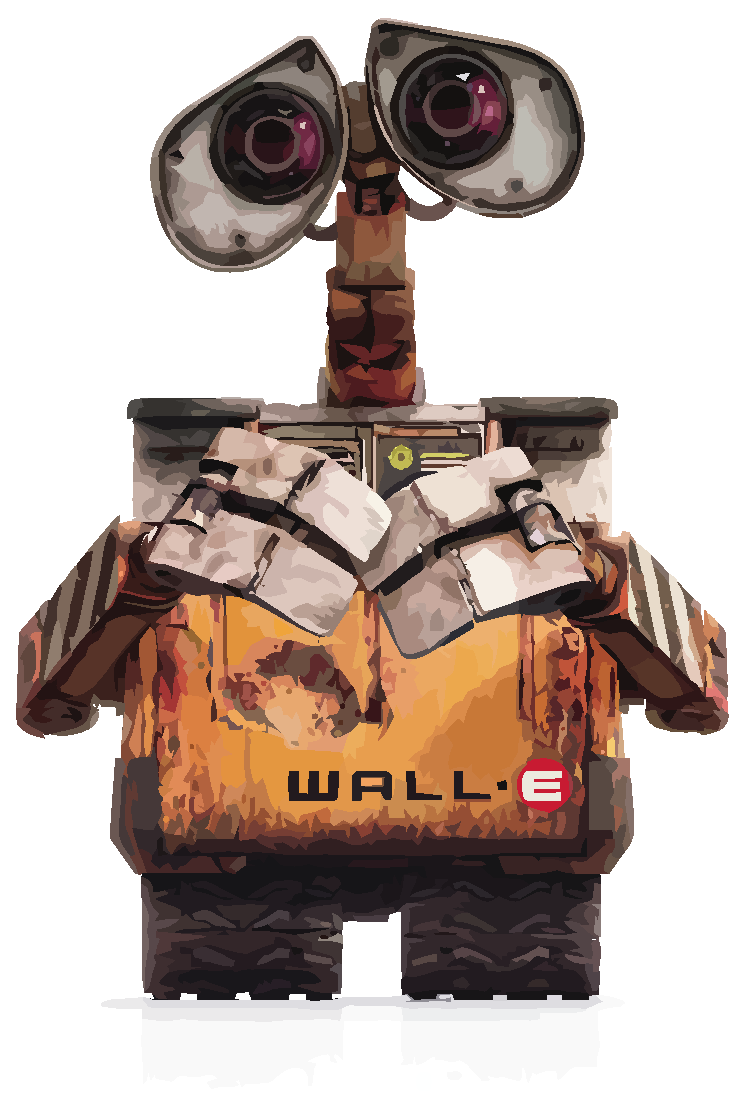
\includegraphics[width=\textwidth]{WallE}
    \caption{Wall-E}
    \label{fig:WallE}
  \end{subfigure}             
  \begin{subfigure}[b]{0.3\textwidth}
    
\includegraphics[width=\textwidth]{minion}
    \caption{Minions}
    \label{fig:Minnion}
  \end{subfigure}
  \caption{Best Animations}
  \label{fig:animations}
\end{figure}


\end{landscape}

%!TEX root = ../thesis.tex
%*******************************************************************************
%****************************** Third Chapter **********************************
%*******************************************************************************
\chapter{Results}
\section{Connectomics}
\subsection{The Central Complex Adult vs Larva}
    \subsection*{Lineages of the Central Complex}

    \subsection*{Protocerebral Bridge}
    In the adult \textit{Drosophila}, the PB comprises two sets of bilaterally symmetric compartments, sometimes referred to as glomeruli 1–9 ~\cite{hulse2021connectome}, positioned at the most posterior-dorsal location possible in the brain.

    These compartments are arranged in a continuous manner medio-laterally, contacting at the midline.
    In the adult, about 600 neurons innervate the PB, organised into hundreds of types (194; \citep{wolff2015neuroarchitecture}) that are split into two main general groups: the columnar neurons (from lineages DM1, DM2, DM3, DM4 and DM6) whose dendrites innervate one or more of the 9 + 9 compartments of the PB~\citep{wolff2015neuroarchitecture}; and the horizontal neurons (also known as horizontal fibers) derived from a single lineage (PBp1; \citep{andrade2019developmentally}) whose axons innervate many or all PB compartments.

    In the adult, the PB receives visual input via relay neurons (POL neurons) conveying information on polarized light, in a highly structured pattern across its compartments that binarizes the continuum of angles of polarized light (\citep{heinze2009transformation}). Then the PB relays this information to the EB compartments.
    % (Table \ref{inputsoutputs});

    In addition to visual input, the adult PB also integrates olfactory inputs \citep{hulse2021connectome}, suggesting that spatial navigation is not unimodal but integrative across multiple sensory modalities.

    In searching for the larval PB, we expected two sets of neurons: columnar and horizontal. In larva, four central complex lineages contribute columnar neurons, a subset of which position their dendrites at a posterior-dorsal location. We could not find a central complex lineage that would contribute horizontal fibers at a posterior-dorsal location necessary to intersect and synapse onto the dendrites of the PB columnar neurons, but we found a larval lineage (DALv1) whose axons are bilateral and project to the appropriate area, and is developmentally related to another central complex lineage (DALv23). This suggests that neurons from non-central complex lineages may be recruited temporarily during the larval period, in a pattern reported so far for the mushroom body (see Discussion; \citep{truman2023metamorphosis}). 


    Among neurons of the DALv1 lineagel, 4 left-right pairs (named HF-PB for "Horizontal Fiber PB") project their axons bilaterally and across the dendrites of the columnar neurons.
    3 of the 4 pairs present an unusual axon configuration: first, they project contralaterally to drop their first output synapses, with the axon then crossing the midline a second time to return back to the same ipsilaterally corresponding location to again drop presynaptic sites .
    This peculiar axon configuration is unique among all neurons of the entire brain of the larva~(\citep{winding2023connectome}) and suggestive of potentially a delay line for comparing left-right sensory inputs.
    The 4th pair first drops presynaptic sites ipsilaterally and then its axon crosses the midline until reaching the corresponding contralateral location to synapse again~(\ref{FigureX}).

    % Relative to the root of their dendritic tree, which is ipsilateral, the first set of output synapses are found contralaterally. Then the axon crosses the midline a second time, returning to the ipsilateral hemisphere to establish more output synapses in a spatially symmetric way to the contralateral set of output synapses.

    The presynaptic outputs of DALv1 neurons are symmetric, in that they contact the same homologous pairs of left-right neurons which are predominantly neurons of the columnar system ~(\ref{FigureX}).
    The axons of these 4 pairs of HF-PB neurons are tiled dorso-ventrally, falling into two bilaterally symmetric groups which we interpret as defining 2 + 2 bilaterally arranged PB compartments, each innervated by 2 pairs of axons. % figure PB compartments

    The dendrites of these 4 pairs of DALv1 neurons (HF-PB) are ipsilateral and dorsal, receiving polysynaptic inputs from vision and olfaction, like in the adult PB~(\citep{hulse2021connectome}). In the larva, we found that these multi-sensory inputs to the horizontal fibers of the PB are mediated by Convergence Neurons (CN-53 and CN-54, among others; \citealp{eschbach2021}) that, as their name indicates, integrate inputs from both Mushroom Body Output Neurons (MBONs) and from the Lateral Horn (LH) such as olfactory and visual PNs \citep{EsbachFushiki2021}). This circuit architecture indicates that sensory inputs arriving to the larval PB will have been modulated or gated by previously established associative memories, with implications for spatial navigation.

    % check for more CNs or other neurons converging onto PB DALv1 dendrites
    %ANSWER: CN35, CN45, CN9 low syn count CN26, CN15
    %as well as from other sensory modalities (Table \ref{sensoryinputs})
    %TODO: describe dendritic and axonic contributions in specific (especially from AL, OL and MB) 
    %2 systems: pattern of input of dendrites of the DALv1 s.
    % MB2ON-175 & 48 & 208 
    % given the PB1-4 compartments, which ones are connected to the MBONs, and the CNs. 175 targets one compartment, 208 targets another.  The pattern is that CNs connect to one compartment of the PB while simultaneously connecting to another CN that connects to the opposite compartment - there could be a gating mechanism. 
    %MB2ON 202 - feedback from the NO to the PB dalv1 


    In the larva, the columnar system consists of neurons from 4 central complex lineages (DPMpm1, DPMpm2, DPMm1 and CM4) that also generate the columnar neurons of the adult (DM1, DM2, DM3 and DM4, correspondingly).
    Larval columnar neurons present small, narrow dendrites circumscribed within the 2 + 2 compartments defined by the axons of the horizontal fibers (DALv1 neurons), with whom they synapse.
    Among the columnar neurons, a subset project their axons directly to the Noduli (NO; \ref{FigureX}), and another subset project directly to the larval Ellipsoid Body (EB; \ref{FigureX}).
    We did not find in the larva columnar neurons whose axons would project to more than one Central Complex neuropil, despite such types being common in the adult~\citep{wolff2015neuroarchitecture; wolff2018; hulse2021connectome}.
    Beyond the canonical columnar neurons projecting to other Central Complex neuropils, we found some whose axons descend to the SEZ or nerve cord~(\ref{FigureX}).



    % TODO Discussion point: this is different than in the adult. 

    % QUESTION: in the adult, are there columnar neurons that descend to the nerve cord? We have them too in larvae Should mention I them. %ANSWER: see figure 63A Hulse et al. supplement 1 PFL -> MDNs (I have a feeling mdn is smth else in adult)

    %In the \textit{Drosophila} larva Electron Microscopy (EM) volume, we found a putative PB situated at the most medial-posterior side of the brain, that receives high levels of visual input and is made of neurons belonging to lineages DM2 (DPMpm1 in the larva) and 8 columnar neurons(4 pairs) belonging to the lineage DALv1. 
    % also - a dopaminergic pathway formed by large field CIVP neurons that relay IDFP signals to the entire PB

    \subsection*{Ellipsoid Body}
    The adult Ellipsoid Body(EB) is a ring-shaped structure situated between the Fan-Shaped Body(FB) and the Mushroom Body horizontal lobes, facing anterodorsally. Its circuit is made up two types of neurons: ring-neurons (derived mainly from the EBAa1/DALv2 and LALv1/BAmv1/2 lineages) that spread their axons across the length of the EB, and reciprocally connected wedge neurons(derived from the DALcl12 lineage) that divide the EB into 16 compartments (aka. wedges)~\citep{omoto2018neuronal}. 

    Its underlying circuit follows the ring attractor architecture (Zhang, 1996) which, as predicted by its anatomy, is shown to yield neural activity in the form of a topological ring in \textit{Drosophila} adult(Seeling \& Jayaraman 2015) with all nodes being connected via inhibitory connections, complemented by local recurrent excitations that maintain activity at each node once they escape inhibition.%(this last sentence is Stanley Heinze).

    The wedge neurons(EPG) form eight wedges around this ring, and project to both hemispheres of the PB, where they connect to two sets of columnar neurons that project back to the EB, forming recurrent loops. These are PEG and PEN neurons. The anatomical offset between EPG and PEN neurons is key to how the fly head direction system translates angular motion into an updated position of the activity bump in the ring attractor. 


    The EB receives visual inhibitory GABAergic inputs, via two parallel pathways for distinct visual information:
    1. Ring neurons that deconstruct the visual environment of the fly; 2. tangential neurons that take in information about body rotations and transnational velocity. The latter receive input in the LAL, output to NO.
    Mechanosensory input also enters the CX via the second order projection neurons to the EB. These neurons code head direction; some proprioceptive input has also been observed 
    ~\citep{hulse2021connectome}. It receives strong inputs from PB, NO and the LAL, and outputs onto the PB.  


    In the 1st instar larva, we found a group of 8 pairs of reciprocally connected neurons from lineage DALcl12 known to produce wedge-neurons in the adult, and categorised these together with one other pair of lineage Dalv23 (which produces ring neurons in adult) with the same connectivity pattern as wedge-neurons. Both their dendrites and axons are very small, and tiled medio-laterally, defining 8 compartments with one single neuron pair contributing to each. These are the intrinsic set of neurons, fully enclosed within the putative larval EB. 

    Similarly, we found one pair of neurons of the BAmv1/2 lineage - known to contribute to ring neurons in adult flies - that receive visual input via PB neurons, and reciprocally interconnects with the previously mentioned wedge-neurons, and whose axons are fully contained within the space defined by the wedge neurons. We categorised these as larval "ring" neurons.

    %We found that a putative structure for the EB in the larva with neurons coming from DALcl12, DALl1 and DALv2(3). This structure seems to receive input from both the LAL and NO(weak) and sends outputs to the PB.

    \subsection*{Fan-Shaped Body}
    % Constituent neurons and the horizontal and vertical compartments they define


    The adult FB is a bilaterally symmetric neuropil anterior to the PB, with well-defined horizontal and vertical components: it has 6 horizontal layers stacked dorso-ventrally that are defined by distinct sets of horizontal neurons(FB tangential neurons); and 9 vertical columns stacked medio-laterally are defined by column-specific columnar neurons. Both horizontal and vertical neurons innervate the FB in a layer- and column-restricted manner ~\citep{heinze2017unraveling}. As one of the biggest CX neuropils, a large variety of lineages contribute to the FB.
    The FB does not receive input along only one clearly defined input pathway, but it is connected to many regions of the surrounding protocerebrum via tangential neurons. 

    There are 2 types of FB tan gential cells: (1)neurons that relay the presence of an attractive odor to the FB, originating in the MB or the LH (learnt or innate valences); (2) neurons that relay sleep drive to the FB, whose activity is mandatory for sleep initiation. 

    The FB columnar neurons, or columnar input cells are known as PFN (PB-FB-NO) and they receive information both in the PB and in the Noduli output cells with dendritic fibers mainly in the FB; 


    There are 5 types of PFNs, they form a p they all receive the same head direction input from the PB, which is integrated with different input signals received in the NO. The PFN outputs are located in distinct layers of the ventral/posterior FB, essentially mapping the noduli layers onto corresponding regions of the FB. PFN cells have a columnar projection pattern that is offset from the default projection scheme between the PB and the central body. This offset generates a head direction bump in the FB that is contralaterally shifted relative to the PB by one column, i.e., 45° of azimuthal space, thus separating right and left cells originating in corresponding PB columns by 90° in the FB.

    The third class of FB cells are interneurons which input and output within the regions of the FB.There are 2 types: FB intrinsic neurons; FB mixed arborisation neurons with additional output branches outside the CX and sometimes input fibers in the PB.


    % Typical synaptic inputs and outputs
    A key feature of the the adult FB is strong innervation by Mushroom Body Output Neurons (MBONs)~\citep{MISSING}. % many, including hemibrain paper
    In addition, the axons of dopaminergic neurons driven by visual inputs innervate the FB~\citep{lin2013comprehensive}.


    % In larva, these are CNs or LHONs:
    %Among the many other inputs to the FB, to remark inputs from the lateral horn (LH)~\citep{hulse2021connectome}, a region known to compute valences from multimodal inputs~\citep{StrutzSachse2014odorquality}. Within the CX, the FB forms bidirectional connections with the PB, the Noduli (NO), and the Lateral Accessory Lobe (LAL). 

    % In larva, now describe FB.b (mostly horizontal fibers like the u-shaped horseshoe neurons) and the FB.d.

    In the larva, we found a number of putative FB horizontal/tangential cells
    originating in lineages known to contribute neurons to the adult FB. Characteristically, most present a bilateral axon closely wrapping around the midline, and an ipsilateral dendrite positioned within the superior dorsal protocerebrum (dorsal anterior neuropil) where they integrate numerous inputs from MBON axons. Among the various neurons with dendrites within this very medial neuropil, we find neurons from lineages known to contribute to the adult FB and whose axons project to the putative larval NO, EB, PB and LAL.

    %We found that a putative FB is also present at the larva, with neurons from the lineages DPMpm1, CM13, DPMpl12 and DPMpm2, and which receives strong synaptic input from MBONs as well as strong reciprocal connectivity with the LAL, the putative NO, and the putative PB. 

    \subsection*{Noduli}
    The noduli are small, bilaterally symmetric spherical neuropils located medially and ventrally to the FB. In the adult \textbf{Drosophila} brain, each hemilateral neuropil is divided in 3 subunits: nodulus 1, 2 and 3 (NO1, NO2, NO3), with NO1 having the highest synaptic density of the three. There are notable variations across insect species, with the number of noduli ranging from two to four per brain hemisphere.
    While the stacked noduli subunits have been referred to as horizontal layers, no vertical subdivisions have been reported for these structures. Therefore there isn't any columnar organisation known.


    The NO neurons present a unique morphology featuring compact, clutchy axons, which set them apart from other CX neurons~\citep{wolff2018neuroarchitecture}~\citep{hulse2021connectome} and greatly ease their identification even in the absence of the typical conspicuous anatomical neuropil region present in adult insects. In the adult fruit fly, these neurons primarily originate in the DM1, DM2 and DM3 lineages~\citep{andrade2019developmentally}.
    %The primary neurites from G9–G6 cross the midline to arborize in the contralateral noduli.


    At the larval stage of this animal, we found a set of neurons with highly compact, clutchy axons situated in the posterior ventral area of the brain, coming from lineages DM1 and DM3, as well as a few other larval lineages, and postulate this as the putative Noduli of the Drosophila larva. 

    %Connectivity
    In the adult \textit{Drosophila} brain, the NO is  interconnected with the EB and the FB, to which they relay information from tangential input neurons via several PB columnar cells such as PEN-neurons(PB-EB-NO; from the Head Direction System) and PFN-neurons(PB-FB-NO)~\citep{wolff2015neuroarchitecture, hulse2021connectome}. The primary NO inputs outside of the CX are from the LAL, these are known as LNO neurons and are suggested to be inhibitory~\citep{wolff2018neuroarchitecture,hulse2021connectome}. LNOs send inputs to and receive feedback from columnar neurons. %TODO check which comumnar neurons. 
    FB tangential neurons make weak reciprocal connections to LNOs and columnar neurons in the NO.
    NO is synaptically interconnected with the other CX neuropils. All columnar neurons (PFNs and PENS) that synapse onto NO (are NO.b) are recurrently connected to the same LNO neurons they receive input from. 

    %TODO: figures with MB and other structures connecting to the CX. especially CNs connecting to every neuropil of the CX.  

    In the putative larval NO, we find that the neurons projecting onto this neuropil receive input from LAL, (LAL.d MB2ON-75)

    %Larval NO - 
    %recurrent connections exist but they are axo-axonic - 
    %most outputs are to MB2ONs, CNs, 10 pars of CNs, mostly MB related neurons. 
    %inputs are mostly multicompartment MBONs. 
    %TODO: no.d s should be the analogus to LNOs. 
    %TODO: find all LAL NEURONS, pk_lal is the volume. LALbs and LALds neuron search : annotation - larval central complex, check everything that is LAL something . look at those that have fullly encolsed synapses -  the lal columns have boh dendrites and axons fully contained in the volumes 
    %VMCc add it to the LAL. that is the LAL 


    %The NO receives inputs from LNO neuron types that innervate accessory structures: LAL, GA, and CRE. 
    % TODO check these set of synaptic connections
    %The majority of NO outputs (of CX columnar neurons) are to other CX columnar neurons (usually of the same type), or to LNO neurons that then provide input to the CX columnar neurons.
    %TODO: check if recurrence is axo axonic - 
    %todo: check if LNO1,2,3 check if they are actually the same as NO.b 
    %NO is synaptically interconnected with the other CX neuropils. All columnar neurons (PFNs and PENS) that synapse onto NO (are NO.b) are recurrently connected to the same LNO neurons they receive input from. 
    %PEN and PFN send output and recieve inputs from NO
    %LNOs mainly send outputs
    %Important comment against NO being an output structure: The only CX columnar neurons that lend some credence to the notion of the NO being an output structure of the CX are the PEN_b neurons, which provide strong inputs to the ExR8 neurons ()


    %%Sensory information
    %Many of these columnar neurons likely also receive input related to the fly’s self-motion in paired structures known as the noduli. 
    In the adult Drosophila, the NO receives optic flow-based self-motion information and wind direction information via the columnar neurons. %an important hub for self-motion information according to physiological and anatomical observations. 
    % TODO In the larva, we find ... 16/21 receive inputs from MBONs, from PB (via 7 PB to noduli neurons, like in the adult), and from FB (some NO.b neurons are also FB.d neurons). 6/21 neurons are columanr neurons that aren't FB.d or PB.d or anything like that.

    %%Larva
    In Drosophila larva, we found a set of neurons with highly compact, clutchy axons situated in the posterior ventral area of the brain - similarly to the adult NO - coming from lineages DM1 and DM3, as well as a few other larval lineages. We observe that these neurons are highly interconnected with the PB and FB,  with strong inputs from 
    PB and strong outputs to FB, and many of these neurons receive inputs in the LAL.
    Their highly distinctive morphology, location as well as similarities in connectivity to the adult noduli, make these neurons an excellent candidate for the putative larval noduli.

    %TO DO: can we see the kind of specific recurrent activity

    \subsection*{Visual input into the Larval Central Complex}
        - 4 graphs showing connectivity between 
    \subsection*{Mushroom Body and the Central Complex}
    \sebsection*{Descending Neurons from CX}
        %catmaid annotation: 
            129 neurons descending to VNC
            93 neurons descending to SEZ
            216 total descending
            layer 1 annotated as: 'cx descending l1' (56 neurons) 25.6\%
            569 second order descending
            layer 2 annotated as: 'cx descending l2' (71 neurons of 569) 12.4\%


\section{Neurotransmitter Identity of Central Complex Neurons}
    \subsection*{DANs Confocal Images}
    \subsection*{GABA and Acetylcholine}
   

\section{Genetic lines for CX neurons}
\section{Optogenetic Activation Screens}
\section{Behavioural Assays - Loss of Function Analysis during light stimulation}
\section{Calcium Imaging Analysis - }





%!TEX root = ../thesis.tex
%*******************************************************************************
%****************************** Third Chapter **********************************
%*******************************************************************************
\chapter{Discussion}
\section{first part}

%\include{Chapter5/chapter5}
%\include{Chapter6/chapter6}
%\include{Chapter7/chapter7}

% Example citation to ensure at least one citation is present
%\cite{exampleReference}



% ********************************** Back Matter *******************************
% Backmatter should be commented out, if you are using appendices after References
%\backmatter

% ********************************** Bibliography ******************************
\begin{spacing}{0.9}

% To use the conventional natbib style referencing
% Bibliography style previews: http://nodonn.tipido.net/bibstyle.php
% Reference styles: http://sites.stat.psu.edu/~surajit/present/bib.htm

%\bibliographystyle{apalike}
%\bibliographystyle{unsrt} % Use for unsorted references  
%\bibliographystyle{plainnat} % use this to have URLs listed in References
\cleardoublepage
%\bibliography{References/references} % Path to your References.bib file


% If you would like to use BibLaTeX for your references, pass `custombib' as
% an option in the document class. The location of 'reference.bib' should be
% specified in the preamble.tex file in the custombib section.
% Comment out the lines related to natbib above and uncomment the following line.

% Ensure your bibliography file is specified in the preamble, e.g.:
% \addbibresource{References/references.bib}

%\printbibliography[heading=bibintoc, title={References}]
%\printbibliography[heading=bibintoc, title={References}]
%\bibliographystyle{plainnat} % or your preferred style

\end{spacing}

% ********************************** Appendices ********************************

\begin{appendices} % Using appendices environment for more functunality

%%!TEX root = ../thesis.tex
% ******************************* Thesis Appendix A ****************************
\chapter{Appendix title example} 

\section*{example}

\subsection*{example}
%\begin{enumerate}
%\item	Download the TeXLive ISO (2.2GB) from\\

%\section{Optogenetic Activation Screens} - this is for appendix
%%!TEX root = ../thesis.tex
% ******************************* Thesis Appendix B ********************************

\chapter{example2}


\end{appendices}

% *************************************** Index ********************************

\printthesisindex % If index is present
\printbibliography[heading=bibintoc, title={References}]


\end{document}
